\documentclass[tikz,border=10pt]{standalone}
\usepackage{tikz}

\begin{document}
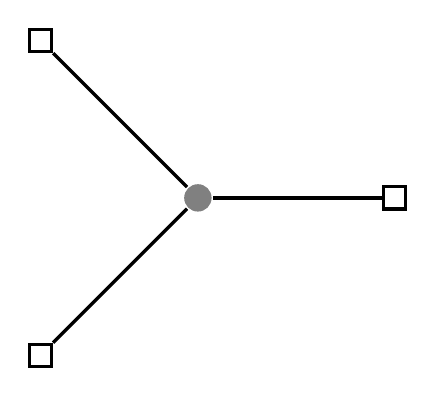
\begin{tikzpicture}[very thick]
    % 定义中心顶点：灰色实心圆，代表可以是黑色(+)或白色(-)的通用相互作用顶点
    \node[circle, fill=gray, inner sep=3.5pt] (v) at (0,0) {};
    
    % 定义外线端点：正方形空心，代表晚期边界上的点（体-边传播子的边界端）
    \node[rectangle, draw, inner sep=4pt] (p1) at (-2, 2) {};
    \node[rectangle, draw, inner sep=4pt] (p2) at (-2, -2) {};
    \node[rectangle, draw, inner sep=4pt] (p3) at (2.5, 0) {};
    
    % 连线：代表体-边传播子 (bulk-to-boundary propagators)
    \draw (p1) -- (v);
    \draw (p2) -- (v);
    \draw (p3) -- (v);
\end{tikzpicture}
\end{document}
